
\documentclass{article}
\usepackage{fullpage, alltt, epsfig, boxedminipage, url}
\twocolumn
\sloppy
\def\nogap{\setlength\itemsep{.0in}\setlength{\parskip}{0in}\setlength{\topsep}{0in}}

\begin{document}
\title{NLTK: Building a Pedagogical Toolkit in Python}
\author{\textbf{Edward Loper}\\
Department of Computer and Information Science\\
University of Pennsylvania, Philadelphia, PA 19104-6389, USA}
\date{}
\maketitle

\begin{abstract}
  
  Teachers of computational classes are faced with the challenge of
  setting up a practical programming component for student assignments
  and projects.  One solution is to construct a broad-coverage
  toolkit, eliminating overhead and leaving students free to think
  about the subject matter rather than low-level programming details.
  This article discusses the criteria and requirements that should
  guide the development of a programming toolkit for courseware, and
  explain how those criteria affected the design and implementation of
  the Natural Language Toolkit (NLTK), a broad-coverage toolkit
  designed for use as computational linguistics courseware.
  
\end{abstract}

%========================= Introduction =========================
\section{Introduction}

Computational linguistics is the study of the application of
computational methods to processing and analyzing natural language.
In an introductory course on computational linguistics, a practical
programming component provides an important tool for teaching students
about these methods.  However, different computational linguistics
domains require a variety of different data structures and functions,
and a diverse range of topics need to be included in the syllabus.
Furthermore, many of the students come from linguistics backgrounds,
and lack strong programming skills.  Therefore, setting up an
easy-to-use practical component can be quite a challenge.

A widespread practice is to employ multiple programming languages,
where each language provides native data structures and functions that
are a good fit for the task at hand.  For example, a typical course
might use Prolog for parsing; Perl for corpus processing; and a
finite-state toolkit for morphological analysis.  This approach allows
the teacher to draw on a wide variety of existing tools, and to avoid
developing a lot of software infrastructure.

But unfortunately, this approach also requires that a significant
portion of the course be devoted to teaching programming languages
instead of computational linguistics.  Furthermore, many interesting
projects span a variety of domains, and would require that multiple
languages be bridged.  For example, a student project that involved
syntactic parsing of corpus data from a morphologically rich language
might involve all three of the languages mentioned above: Perl for
string processing; a finite state toolkit for morphological analysis;
and Prolog for parsing.  

These same challenges face the teacher of any computational subject
that requires a strong practical component (such as computational
biology).  In this article, we discuss the issues involved in building
a broad-coverage pedagogical toolkit; and show how we addressed those
issues in the Natural Language Toolkit (NLTK), a Python-based
programming toolkit developed in conjunction with a course we have
taught at the University of Pennsylvania.

%========================= Applications =========================
\section{Applications}

Before designing a pedagogical toolkit, it is important to consider
the uses that it will be put to.  We divided the toolkit's applications
into three basic categories: assignments, in-class demonstrations, and
advanced projects.

\subsection{Assignments}

We wanted the toolkit to support homework assignments of varying
difficulty and scope.  In the simples assignments, students would use
and experiment with existing components.  The toolkit should provide
broad coverage, to allow assignments to be created for a wide variety
of topics.  Once students became more familiar with the toolkit, they
could be asked to make minor changes or extensions to existing
components.  Finally, students can be asked to create complete systems
by combining existing components.

\subsection{In Class Demonstrations}

In class graphical demonstrations can be powerful tools for explaining
concepts and algorithms.  Interactive demonstration tools can be used
to display relevant data structures, and to show the step-by-step
execution of important algorithms.  It should be possible to modify
both data structures and control flow during the demonstration, in
response to questions from the class.  Finally, any graphical
demonstration tools should be accessible to the students.  This allows
students to experiment at home with the algorithms that they have seen
presented in class.

\subsection{Advanced Projects}

The toolkit should provide students with a flexible framework for
advanced projects.  Typical projects might involve implementing a new
algorithm, developing a new component, or adding support for a new
task.

%========================= Requirements =========================
\section{Requirements}

Based on these three applications, we defined the following set of
requirements for the toolkit's design, listed in decreasing of 
importance.

\paragraph{\textit{Ease of Use.}} The primary purpose of the toolkit is
to allow students to concentrate on building natural language
processing (NLP) systems.  The more time students must spend learning
to use the toolkit, the less useful it is.

\paragraph{\textit{Consistency.}} The toolkit should use consistent data
structures and interfaces.

\paragraph{\textit{Extensibility.}} The toolkit should easily
accommodate new components, whether those components replicate or
extend the toolkit's existing functionality.  The toolkit should be
structured in such a way that it is obvious where new extensions would
fit into the toolkit's infrastructure.

\paragraph{\textit{Documentation.}} The toolkit, its data structures,
and its implementation all need to be carefully and thoroughly
documented.  All nomenclature must be carefully chosen and
consistently used.

\paragraph{\textit{Simplicity.}} The toolkit should structure the
complexities of building NLP systems, not hide them.  Therefore, each
class defined by the toolkit should be simple enough that a student
could implement it by the time they finish an introductory course in
computational linguistics.

\paragraph{\textit{Modularity.}} The interaction between different
components of the toolkit should be kept to a minimum, using simple,
well-defined interfaces.  In particular, it should be possible to
complete individual projects using small parts of the toolkit, without
worrying about how they interact with the rest of the toolkit.  This
allows students to learn how to use the toolkit incrementally
throughout a course.  Modularity also makes it easier to change and
extend the toolkit.

\subsection{Non-Requirements}

It is equally important to specify properties that are \emph{not}
expected of the toolkit:

\paragraph{\textit{Comprehensiveness.}} Although the toolkit should
provide broad coverage, it is not intended to provide a comprehensive
set of tools.  Indeed, there should be a wide variety of ways in which
students can extend the toolkit.

\paragraph{\textit{Efficiency.}} The toolkit does not need to be highly
optimized for runtime performance.  However, it should be efficient
enough that students can use their NLP systems to perform real tasks.

\paragraph{\textit{Cleverness.}} Clear designs and implementations are
far preferable to ingenious yet indecipherable ones.

%========================= Why Python? =========================
\section{Why Python?}

The first step in designing a pedagogical toolkit is choosing a
suitable programming language.  Python is especially well suited to
the task, for a number of reasons:

\begin{itemize}
\item Python offers a shallow learning curve; it was designed to be
  easily learnt by children \cite{cp4e}.  This ensures that students
  without a strong computer science background can quickly get up to
  speed.
  
\item Python code is exceptionally readable, with transparent syntax
  and semantics; it has been praised as ``executable pseudocode.''
  Examples are therefore easy for students to follow.  Furthermore,
  students can learn by looking at the toolkit's source code, and not
  just by using it.
  
\item As an interpreted language, Python is suitable for interactive
  exploration.  Students can experiment with the toolkit, and get
  immediate feedback.
  
\item Python's light-weight object oriented system makes it easy to
  encapsulate data and methods in classes, without forcing students to
  use them where they're not necessary.
  
\item Python's recently added generator syntax makes it easy to create
  interactive implementations of algorithms.  These interactive
  implementations can be used to ``step through'' the algorithm,
  examining how its state changes as the algorithm progresses.
  
\item Python's extensive standard library provides a great deal of
  power, when needed.  For example, the \texttt{Numeric} library can
  be used to implement computationally intensive algorithms that would
  otherwise be too slow if implemented in Python.
\end{itemize}

%========================= Design =========================
\section{Design}

NLTK is implemented as a large collection of minimally interdependent
modules, organized into a shallow package hierarchy.  A set of core
modules defines basic data types that are used throughout the toolkit.  
The remaining modules are \emph{task modules}, each devoted to an
individual natural language processing task.  For example, the
\texttt{nltk.parser} package encompasses to the task of
\emph{parsing}, or deriving the syntactic structure of a sentence; and
the \texttt{nltk.tokenizer} module is devoted to the task of
\emph{tokenizing}, or dividing a text into its constituent parts.

\subsection{Core Data Types}

\subsubsection{Token}

To maximize interoperability between different modules, we use a
single class to encode information about natural language texts -- the
\texttt{Token} class.  Each \texttt{Token} instance represents a
single unit of text, such as a word, sentence, or document; and is
defined by (partial) mapping from property names to values.  For
example, the \texttt{TEXT} property is used to encode a token's text
content; and the \texttt{TAG} property is used to encode a word
token's part-of-speech tag.  The \texttt{LOC} property is used to
specify the location of a token in its containing text.  This location
can be used to decide whether two \texttt{Token} objects refer to the
same piece of text or not.

Natural language processing tasks are formulated as transformations on
\texttt{Tokens}.  In particular, each processing task takes a token,
and extends it to include new information.  Typically, these
modifications are \emph{monotonic}; in other words, new information is
added but existing information is not deleted or modified.  Thus,
tokens serve as a sort of \emph{blackboard}, where information about a
piece of text can be incrementally built up.  This architecture
contrasts with the more typical \emph{pipeline} architecture, where
each processing task's output discards its input information.  We
chose the ``blackboard'' approach over the ``pipeline'' approach
because it allows more flexibility when combining tasks into a single
system.  In particular:

\begin{itemize}
\item Since no information is discarded, and all information is
  accessed the same way, students don't need to worry about
  ``threading'' information through the system to the tasks that need
  it.
  
\item Because every processing tasks has the same basic interface, the
  order in which processing tasks are applied can be easily modified.  

\item Monotonic modification allows tasks to transform to a piece of a
  structure without copying the remaining structure.
  
\item Monotonic modification ensures that the information seen by
  different tasks is consistent.
\end{itemize}

\noindent The primary disadvantage of the ``blackboard'' approach is
that it can be inefficient.  In particular, token properties are not
deleted even if they will not be used.  But for a pedagogical toolkit,
flexibility is more important than efficiency; and if necessary, the
unused properties can be explicitly deleted.

\subsubsection{Token Subclasses}
It is often useful to use a token as a key in a dictionary or an
element in a set.  NLTK therefore defines a hashable and immutable
token subclass, \texttt{FrozenToken}.

A number of other subclasses are used to support special token types.
For example, the \texttt{TreeToken} class adds methods for performing
tree manipulation operations; and the \texttt{ParentedTreeToken} class
automatically maintains consistent parent pointers for tree
structures.

\subsubsection{Other Core Data Types}

In addition to the \texttt{Token} class, NLTK defines a variety of
data types that are useful for language processing.  For example, the
\texttt{nltk.probability} module defines classes that encode frequency
distributions and probability distributions, including conditional
distributions and a variety of statistical smoothing techniques; the
\texttt{cfg} module defines classes for encoding context free grammars
and probabilistic context free grammars; and the \texttt{corpus}
module defines classes for reading and processing standard language
processing corpora.

\subsection{Task Modules}

Task modules define individual natural language processing tasks, such
as parsing and tokenizing.

\subsubsection{Task Classes}

Each processing task algorithm is encoded as a class.  For example,
the \texttt{ChartParser} and \texttt{Recursive\-Descent\-Parser} classes
each define a single algorithm for parsing a text.  Although it might
seem unintuitive at first, there are a number of advantages to using a
class (rather than a function) to encode an algorithm.  First, all
algorithm-specific options can be passed to the constructor, allowing
a consistent interface for actually applying the algorithms.  Second,
a number of algorithms need to have their state initialized before
they can be used.  For example, the \texttt{NthOrderTagger} class must
be initialized by training on a tagged corpus before it can be used.
Finally, subclassing can be used to create specialized versions of a
given algorithm.

\subsubsection{Task Interfaces}

In order to provide a formal specification of the interface for a
given task, each task module defines an \emph{interface} for its task.
These interfaces are encoded interfaces as skeletal base classes that
use docstrings to specify each method's behavior.  Using epydoc, these
docstrings can be inherited by derived classes \cite{epydoc}.  Each
required method raises an \texttt{AssertionError}, since any valid
implementation of the interface must override it; and any optional
methods raise \texttt{Not\-Implemented\-Error}.  Interfaces are
distinguished by naming them with a trailing capital ``\texttt{I},''
such as \texttt{ParserI} and \texttt{TokenizerI}.

Each interface defines a single \emph{action method}, which actually
performs the task defined by the interface.  For example, the
\texttt{ParserI} interface defines the \texttt{parse} method; and the
\texttt{Tokenizer} interface defines the \texttt{tokenize} method.
When appropriate, an interface will also define \emph{extended action
  methods}, which provide variations on the basic action method.  For
example, the \texttt{ParserI} interface defines the \texttt{parse\_n}
method, which finds all possible structures for a given sentence; and
the \texttt{TokenizerI} interface defines the \texttt{xtokenize}
method, which outputs an iterator over subtokens instead of a list of
subtokens.

\subsection{In-Class Demonstrations}

We used the Tkinter toolkit \cite{tkinter} to create several tools
that can be used to demonstrate the algorithms implemented by NLTK.
We chose Tkinter because it is almost universally distributed with
Python; it is therefore possible for students to play with the
demonstration tools at home.  These GUI demonstrations are built on
top of the basic task implementations; and use generators to step
through the algorithm's operations.  The demonstration tools also
modification and manual control over the basic algorithm.  This lets
teachers to use the tools to highlight specific points about an
algorithm; and makes it easy for students to experiment with the
algorithm at home.  Figure \ref{fig:chart} shows the chart parsing
demo, which is used to illustrate a variety of different chart parsing
algorithms.

\begin{figure}
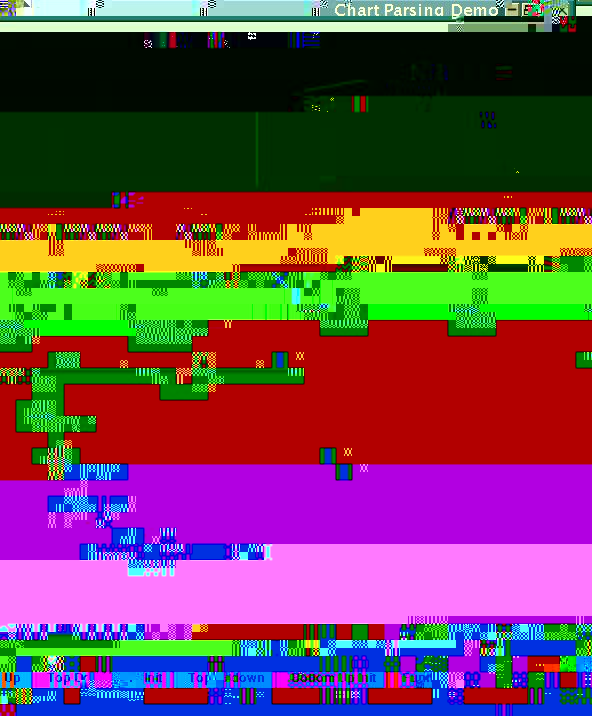
\epsfig{file=chart.eps, width=8cm}
\caption{The Chart Parsing Demo}
\label{fig:chart}
\end{figure}


\section{Conclusions}

NLTK is a broad-coverage toolkit that provides a simple, extensible,
uniform framework for assignments, projects, and class demonstrations.
It is well documented, easy to learn, and simple to use.

NLTK is unique among computational linguistics tools in its
combination of three factors.  First, it was deliberately designed as
courseware and gives pedagogical goals primary status.  Second, its
target audience consists of both linguists and computer scientists,
and it is accessible and challenging at many levels of prior
computational skill.  Finally, it is based on an easy-to-learn and
easy-to-read programming language supporting rapid development and
literate programming.

We plan to continue extending the breadth of materials covered by the
toolkit.  We also plan to increase the number of algorithms
implemented by some of the existing modules, such as the text
classification module.

NLTK is an open source project, and we welcome any contributions.
Readers who are interested in contributing to NLTK, or who have
suggestions for improvements, are encouraged to contact the author.

\section{Acknowledgements}

We are indebted to our students for feedback on the toolkit, and to
all the independent contributors who helped add new content to the
toolkit.  We are grateful to Mitch Marcus and the Department of
Computer and Information Science at the University of Pennsylvania for
sponsoring the original development of the toolkit.

\nocite{nltk}
\bibliographystyle{apalike}
\bibliography{pycon}

\end{document}
